% SPDX-License-Identifier: GPL-2.0-or-later
% Copyright 2018 Association Prologin <info@prologin.org>
% Copyright 2018 Thibault Allançon

%LaTeX Document
\documentclass[a4paper,twoside,12pt]{article}
\usepackage{xltxtra}
\usepackage{url}
\usepackage{caption}
%\usepackage{lettrine}
\usepackage{wrapfig}
\usepackage{longtable}
\usepackage{booktabs}
\setromanfont[Mapping=tex-text]{TeX Gyre Pagella}
\setsansfont[Mapping=tex-text]{DejaVu Sans}
\setmonofont[
  Mapping=tex-text,
%  Scale=0.85,
  AutoFakeSlant,
  BoldItalicFeatures={FakeSlant}]{Inconsolata}
%\newfontfamily{\A}[Scale=0.85]{DejaVu Sans} % TODO find a free Arial/Helvetica equivalent
%\newfontfamily{\J}[Scale=0.85]{Hiragino Kaku Gothic Pro}
%\newfontfamily{\P}[Scale=0.85]{Palatino}
\usepackage{soul} % Pour barrer
\usepackage{textcomp} % Pour les trademarks

%%%%%%%%%%%%%%%%%%%%%%%%%%%%%%%%
%%         BEGIN FIXME         %
%%%%%%%%%%%%%%%%%%%%%%%%%%%%%%%%
\def\plongday{Samedi}
\def\pday{19}
\def\pmonth{mai}
\def\pyear{2018}

\def\ptitle{\textsc{Penguins in Black}} %% Subject's main title
\def\psubtitle{\color{red}TOP SECRET//SI//ORCON//NOFORN} %% Subject's sub title

\def\plogo{prologin2018.pdf} %% Logo FIXME
\def\psubjectpicture{logofinale_inv.pdf} %% Picture to be displayed FIXME
%% on its own page

%%%%%%%%%%%%%%%%%%%%%%%%%%%%%%%%
%%         END FIXME           %
%%%%%%%%%%%%%%%%%%%%%%%%%%%%%%%%


%%%%%%%%%%%%%%%%%%%%%%%%%%%%%%%%%%%%%%%%%%%%%%%%%%%%%%%%
%%              DO NOT EDIT PAST THIS LINE            %%
%%%%%%%%%%%%%%%%%%%%%%%%%%%%%%%%%%%%%%%%%%%%%%%%%%%%%%%%











%\documentclass[a4paper,twoside,12pt]{book}

\usepackage[french]{babel} % TODO switch to polyglossia?
\usepackage{geometry}
\usepackage{multicol}
\usepackage{fancyhdr}
\usepackage{listings}
\usepackage{array}
\usepackage{color}
\usepackage{caption}
\usepackage{subcaption}
\usepackage{amsmath}
\usepackage{tikz}

\def\pdate{\plongday{} \pday{} \pmonth{} \pyear{}}
\def\tightlist{} % fix for pandoc

\definecolor{colIdentifier}{gray}{0}
\definecolor{colKeys}{rgb}{0,0,0.6}
\lstset{
    extendedchars=false,
    showstringspaces=false,
    escapeinside=@@,
%    keywordstyle=\color{blue},
%    commentstyle=\color[rgb]{0.133,0.545,0.133},
    columns=flexible,
    language=C++,
    tabsize=2,
    basicstyle=\ttfamily\NoAutoSpacing
%    numbers=left,
%    frame=lines
}
\lstnewenvironment{lst-c++}{%
\lstset{%
language=C++
}}{}

\newcommand{\wfig}[2]{
}


\captionsetup{justification=centering}

%\renewcommand\ttdefault{cmtt}

\newcommand{\functitle}[1]{%
\vspace{0.5cm}
$\bullet$ \underline{\textbf{#1}}
}

%\NoAutoSpaceBeforeFDP
\geometry{bindingoffset=5mm,hmarginratio=1:1,heightrounded,headheight=15pt,bmargin=3cm}

\setcounter{tocdepth}{2}

\makeindex

\begin{document}
\pagestyle{empty}
\sloppy

\lhead[\thepage]{\nouppercase \leftmark}
\rhead[\textsl{Prologin \pyear{}} --- Sujet de la finale]{\thepage}
\cfoot{\color{red}TOP SECRET//SI//ORCON//NOFORN}

\sethlcolor{black}

% Couverture =========================================================
\begin{titlepage}
\begin{center}
~\includegraphics[width=\linewidth]{\plogo}\\
\vspace{5cm}
\Huge
\textbf{\ptitle{}}

\vspace{1cm}

\Large
\textbf{\psubtitle{}}

\vspace{2cm}

\normalsize
\textnormal Sujet de la finale du Concours National d'Informatique\\
\pdate\\

\vspace{2cm}
\hl{Never gonna give you up. Never gonna let you down.}

\hl{Never gonna run around and desert you.}
\end{center}

\vspace{3cm}
\hl{Never gonna make you cry.}

\end{titlepage}

\small

% Sommaire ===========================================================
\cleardoublepage
\tableofcontents

\normalsize

% Corps ==============================================================
%\cleardoublepage
\setcounter{page}{1}
\pagestyle{fancy}
\parskip=6pt plus 3pt

\newpage
\vspace{4cm}
\begin{center}\includegraphics[height=14cm]{\psubjectpicture}\end{center}

\newpage

\section{Contexte}
\subsection{Épisode 1 : Crise}
\hfill \textit{Maubeuge, Nord, jeudi 17 mai 2018}

Cela fait maintenant trois ans que vous êtes employé dans le bureau des
IeN\footnote{\emph{Individus en Noir}\texttrademark.}.  Affecté depuis la moitié
de ce temps dans les bureaux grisâtres du Nord Pas-de-Calais\footnote{La
délocalisation affecte tous les secteurs.}, vous pensiez que votre carrière se
limiterait à servir le café à des quadragénaires pédants. 

Pourtant, ce matin, vous notez une agitation certaine dans les locaux du 4, Rue
du Trieu Mouton, Maubeuge, 59600, FRANCE.  Effectivement, alors que vous
naviguiez entre les bureaux Ikea pour déposer un latte - tiède, avec deux sucres
- sur la grosse patte gélatineuse de Beauté, l'alien aux télécommunications,
vous surprenez des cris provenant directement du bureau du Directeur, D. Les
têtes se dressent, curieuses, d'un peu partout de l'open space. Malgré votre
professionnalisme à toute épreuve, vous ne pouvez vous empêcher de jeter un œil,
vous aussi. À travers les stores entrouverts du bureau, vous voyez le directeur
et J\footnote{De son vrai nom Joseph Marchand.}, un de vos collègues affectés au
terrain\footnote{Promotion dont vous rêvez chaque soir : ils ont beaucoup plus
de RTT.}, engagés dans une discussion animée dont vous entendez quelques bribes
: apparemment, il se passe quelque chose de très grave impliquant le Pôle Sud,
des aliens, et le menu de la cantine.

Le ton monte et, inquiet, vous fixez franchement les deux hommes - cela fait
maintenant trop longtemps que le cuisinier essaye de tous vous empoisonner -
quand ceux-ci se détournent brusquement vers vous. Ils vous regardent, vous les
regardez, puis vous vous voyez soudainement convoqué par un signe sec du
Directeur. Avec un courage que vos collègues saluent en murmurant, vous entrez.

\begin{itemize}
\item[-] Un petit café ?
\item[-] Ça vous dirait de diriger une équipe ?
\item[-] Ah ben oui, pourquoi pas.
\end{itemize}

Silence.

\begin{itemize}
\item[-] Bon, j'ai une idée.
\end{itemize}

Et sur cette déclaration étonnante, J plonge les mains dans la poubelle et en
extirpe une affiche recouverte de manchots\footnote{Et non pas de pingouins.},
où s'étale en grand le mot suivant : \emph{Prologin}.

\subsection{Épisode 2 : Les PiB}
\hfill \textit{Kremlin-Bicêtre, Île-de-France, samedi 19 mai 2018}

Voilà comment vous vous êtes retrouvés dans le bureau des
PiB\footnote{\emph{Prologin in Black}\texttrademark}, sous-équipe du
sous-sous-secteur du Kremlin-Bicêtre.

Le Président, B, vous explique la situation.

\begin{itemize}
    \item[-] Le Département Administratif des Déplacements Aliens\footnote{Le
        \emph{DADA} est très à cheval sur les acronymes.} est formel : une large
        invasion alien se prépare.
    \item[-] Mais pourquoi ?
    \item[-] On ne le sait pas vraiment.\footnote{D'après les rumeurs, une
        sombre histoire de clafoutis.}
\end{itemize}
B balaye toutes vos protestations dubitatives d'un mouvement ample de la main.
\begin{itemize}
    \item[-] En tout cas, une chose est certaine : un groupe d'aliens débarquera
        en repérage au Pôle Sud. Il faut absolument en capturer avant qu'ils ne
        repartent pour déterminer quel est leur plan, et empêcher l'invasion.
        C'est pour cela que nous avons décidé de mettre nos meilleurs agents
        dessus : les manchots.
    \item[-] Les quoi ?
    \item[-] Les manchots.
    \item[-] Pardon ?
\end{itemize}

B soupire et tire de sa poche une petite photographie froissée. Vous discernez
dessus une silhouette replète, ronde et toute douce, ornée d'une paire de
lunettes de soleil sur son adorable petit bec.

\begin{itemize}
    \item[-] Aaaaw.
    \item[-] Détrompez-vous, ils sont redoutables. Leur vitesse n'a aucun égal
        sur la glace.
    \item[-] Bon, dans ce cas, pourquoi on est là ?
    \item[-] Les manchots ont un problème majeur, explique B en ajustant ses
        lunettes. Ils sont très, très stupides. Ils auront besoin de quelqu'un
        pour leur expliquer quoi faire.
\end{itemize}

Et d'un geste dramatique, B montre de la main les recrues pullulant dans la
cour.

\newpage
\subsection{Épisode 3 : Les joies de l'administration française}
\hfill \textit{Pôle Sud, samedi 19 mai 2018}

Vous sortez vos jumelles et les pointez droit vers la banquise jusqu'à retrouver
les petits points noirs : les quatre manchots qui composent votre équipe.
Cependant, vous déchantez vite. Un peu plus haut, vous repérez quatre petits
points noirs supplémentaires : les aliens, déjà !? Non. D'autres
pingouins\footnote{Pardon. D'autres \emph{manchots}.}. Mais d'où ?

Irrité, vous appelez aussitôt votre supérieur hiérarchique direct.

\begin{itemize}
    \item[-] À quoi ça rime ? Pourquoi on est deux équipes au même endroit ?
    \item[-] Euuuuuh... Attendez.
\end{itemize}

Petite musique d'ascenceur.

\begin{itemize}
    \item[-] Bah en fait, euh, ben, il y a eu une erreur.
    \item[-] Une erreur ?
    \item[-] On a peut-être, ou peut-être pas, envoyé deux équipes sur la même
        partie de la banquise...\footnote{Cf. le titre}
\end{itemize}

Vous raccrochez, et réfléchissez. Que devriez-vous faire ? Laisser l'autre
équipe s'en occuper, quitte à perdre votre travail ? Ou profiter de cette
compétition pour briller aux yeux des PiB ? Le choix est vôtre.\footnote{En
fait, si vous êtes toujours là, vous n'avez plus vraiment le choix.}


\newpage
\section{Instructions de mission}\label{instructions-de-mission}

\subsection{Banquise}\label{banquise}

Dans le cadre de votre mission, vous serez envoyé au Pôle Sud, sur une
partie de la banquise où nos services de renseignements ont indiqué que
les premiers repérages aliens auront lieu. La banquise est représentée
par une grille carrée de 25 cases de côté.

\begin{figure}[!h]
    \centering
    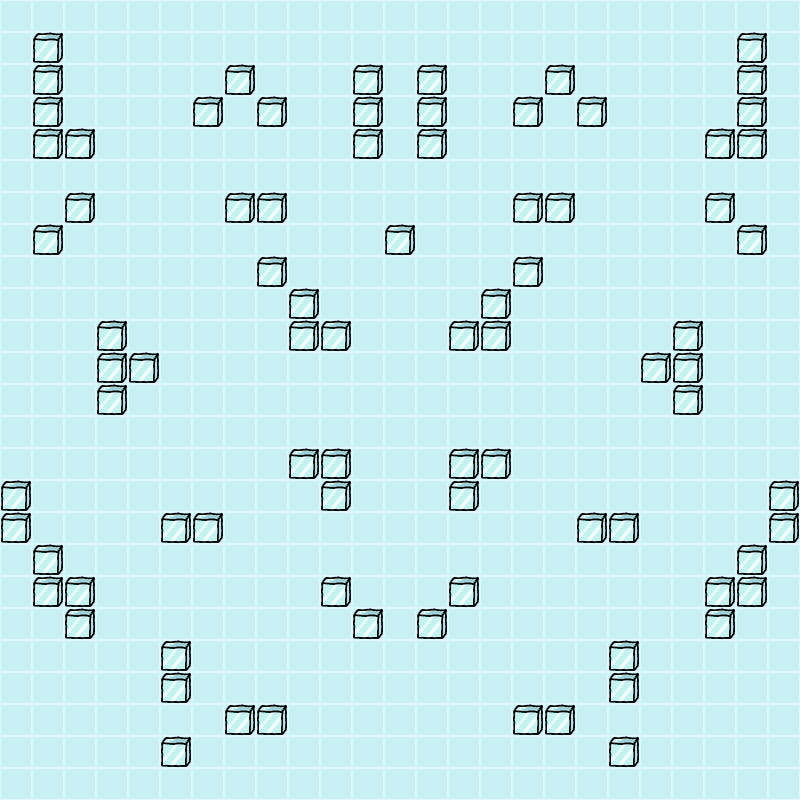
\includegraphics[width=8cm]{img/map.png}
    \caption*{Une partie de la banquise.}
\end{figure}

Une position sur la banquise est notée à l'aide d'un couple $(ligne,
colonne)$, où $0 \leq ligne, colonne < 25$.

\subsubsection{Cases}\label{cases}

Chaque case de la banquise est soit libre, soit un mur de glace. Les
murs sont des obstacles et bloquent tout déplacement sur la case.

Une case libre peut contenir un alien ainsi qu'un agent. Un agent peut
être sur la même case qu'un alien, en revanche il est impossible d'avoir
plusieurs agents ou plusieurs aliens sur une même case.

\subsubsection{Agents}\label{agents}

Les deux recrues PiB ont à leur disposition quatre agents, numérotés de
0 à 3. Ces derniers sont considérés comme des obstacles, et bloquent
donc tout déplacement sur la case.

\begin{figure}[!h]
    \centering
    
\includegraphics[width=1.5cm]{img/penguin}
    \caption*{Un agent PiB.}
\end{figure}

\subsubsection{Aliens}\label{aliens}

Des aliens débarqueront sur la banquise à des positions précises de la
carte, pendant un certain nombre de tours afin d'accomplir leur mission
de reconnaissance, avant de repartir sur leur planète d'origine. De
plus, les aliens n'envahissent jamais plusieurs fois le même endroit sur
la banquise.

\begin{figure}[!h]
    \centering
    
\includegraphics[width=1.5cm]{img/alien}
    \caption*{Un alien menaçant.}
\end{figure}

Pour capturer un alien, un agent doit être sur la case pendant au moins
3 tours. L'alien capturé disparaît de la banquise, et des échantillons
d'analyse sont envoyés instantanément au QG des PiB, l'agent peut donc
continuer sa mission. Si l'agent quitte la case, ne serait-ce qu'un
instant (en se déplaçant ou alors en étant poussé par un agent), la
capture devra reprendre de \textbf{zéro}.

\begin{figure}[!h]
    \centering
    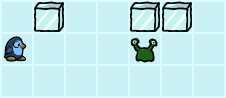
\includegraphics[width=4.5cm]{img/alien_capture1}
    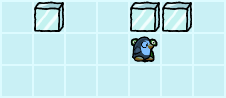
\includegraphics[width=4.5cm]{img/alien_capture2}
    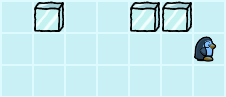
\includegraphics[width=4.5cm]{img/alien_capture3}
    \vspace{-0.3cm}
    \caption*{(3 tours)}
    \caption*{Un agent qui capture un alien, puis continue sa mission.}
\end{figure}

Les aliens ne sont pas assez habitués à la glace pour se déplacer sur
la banquise. Ils se contenteront donc pour leur mission de repérage de
rester fixes par rapport à leurs lieux d'invasion. En revanche, les
aliens ne sont pas des obstacles : faisant des efforts admirables pour
éviter les agents - contrairement aux murs, qui sont davantage
récalcitrants - ils se contorsionneront et esquiveront de leur mieux :
ils ne bloquent donc pas le déplacement des agents.

\begin{figure}[!h]
    \centering
    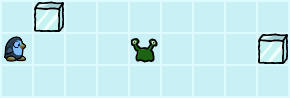
\includegraphics[width=5cm]{img/alien_not_obstacle1}
    \hspace{0.5cm}
    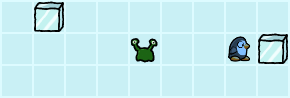
\includegraphics[width=5cm]{img/alien_not_obstacle2}
    \caption*{Les aliens ne sont pas des obstacles.}
\end{figure}

\newpage
\subsection{Déroulement d'un tour}\label{duxe9roulement-dun-tour}

Il y a 100 tours par partie, numérotés de 0 à 99. Pendant un tour les
recrues jouent alternativement. Les invasions ou départs d'aliens ont
toujours lieu en début de tour avant les actions des joueurs. Par
exemple, si un alien envahit la banquise au tour 10, pour une durée de 3
tours, alors il sera présent aux tours 10, 11 et 12 et repartira au tout
début du tour 13. En revanche, la capture des aliens se fait toujours à
la fin du tour, lorsque les deux recrues ont fini de jouer.

Tous les agents se voient attribuer 8 points d'action au début de chaque
tour. Ces points ne sont utilisables que durant ce tour et sont
spécifiques à un agent (il est donc impossible de transférer des points
d'un agent à un autre). Les points vous permettent d'effectuer les
actions ci-dessous.

\subsubsection{Actions}\label{actions}

\paragraph{Déplacer}\label{duxe9placer}

Vous pouvez déplacer un agent vers une case libre adjacente dans la
direction de votre choix (nord, sud, est, ouest). Cette action coûte 1
point d'action à l'agent.

\paragraph{Glisser}\label{glisser}

Un agent peut s'élancer fougueusement sur la banquise, directement sur
le ventre, dans une certaine direction, ce qui le propulse jusqu'à ce
qu'il heurte un obstacle (un autre agent ou un mur). L'action coûte 3
points d'action.

\begin{figure}[!h]
    \centering
    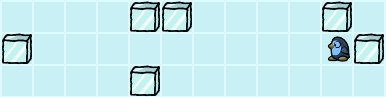
\includegraphics[width=7cm]{img/slide1}

    \vspace{0.5cm}
    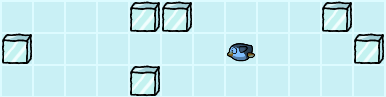
\includegraphics[width=7cm]{img/slide2}

    \vspace{0.5cm}
    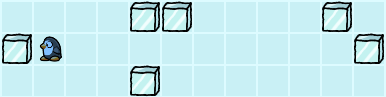
\includegraphics[width=7cm]{img/slide3}

    \caption*{Un agent qui glisse vers l'ouest.}
\end{figure}

\newpage
\paragraph{Pousser}\label{pousser}

Il est possible de pousser un autre agent (allié ou ennemi) si ce
dernier est sur une case adjacente à l'un de vos propres agents. Le
pousser dans une direction le fait glisser jusqu'à ce qu'il rencontre un
obstacle. Pousser un agent coûte 5 points d'action.

\begin{figure}[!h]
    \centering
    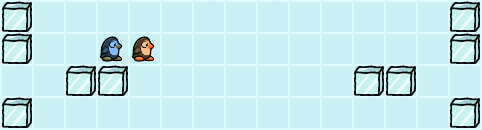
\includegraphics[width=7cm]{img/push1}

    \vspace{0.5cm}
    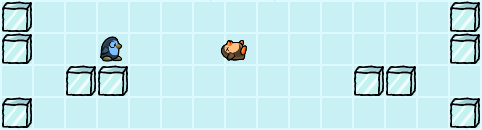
\includegraphics[width=7cm]{img/push2}

    \vspace{0.5cm}
    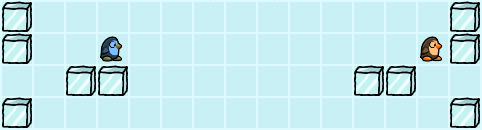
\includegraphics[width=7cm]{img/push3}

    \caption*{L'agent bleu pousse l'agent rouge.}
\end{figure}

À nouveau, les aliens font tout leur possible pour esquiver les agents,
vous ne pouvez donc pas les pousser (ce n'est pas pour rien qu'il faut 3
tours pour les capturer !).

\paragraph{Débug}\label{duxe9bug}

Pour vous permettre de débugger votre intelligence artificielle, il est
possible de placer des drapeaux de débug de trois couleurs différentes
sur la carte que vous pourrez ainsi voir dans l'interface de la
simulation. Cette action ne coûte aucun point d'action.

\begin{figure}[!h]
    \centering
    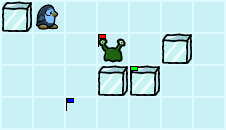
\includegraphics[width=5cm]{img/debug_flags}
    \caption*{Drapeaux de débug.}
\end{figure}

\subsubsection{Score}\label{score}

Chaque alien capturé vous rapporte un certain nombre de points en
fonction de l'alien, selon son espèce, le danger brut qu'il représente,
et ses opinions politiques. La recrue ayant accumulé le plus de points à
la fin de la partie rejoindra les rangs des \emph{Prologin in
Black}\texttrademark pour lutter contre les invasions intergalactiques.

\subsubsection{Format de la carte}\label{format-de-la-carte}

La carte de la banquise est représentée dans un fichier texte qui suit
le format suivant :

\begin{verbatim}
banquise ASCII
positions de depart agents joueur 1
positions de depart agents joueur 2
description des aliens
\end{verbatim}

La représentation ASCII de la banquise est constituée de « \texttt{.} » pour
une case libre et « \texttt{X} » pour un mur.

Pour chaque joueur, quatre lignes, une par agent, indiquent la position
de départ d'un agent sous la forme \texttt{ligne\ colonne}.

La description des aliens commence par un nombre sur une seule ligne
indiquant le nombre d'aliens qui envahiront la banquise durant la
partie. Chaque ligne précise ensuite les caractéristiques d'un alien :
\texttt{position\_ligne\ position\_colonne\ points\_capture\ tour\_invasion\ duree\_invasion}


\newpage
\section{Tournois}

\subsection{Tournois intermédiaires}

Afin de vous aider à perfectionner vos algorithmes, des tournois intermédiaires
vous seront proposés toutes les six heures environ. Ces matchs n'ont absolument
aucune influence sur le classement final, mais sont néanmoins à prendre au
sérieux car ils vous permettront de vous situer par rapport aux autres
joueurs, de connaître vos ennemis, vos points forts et vos faiblesses, et vous
donneront des pistes pour vous améliorer pendant la finale.

Les tournois se dérouleront aux horaires suivants :

\begin{itemize}
    \item Samedi 15~h~42 (tournoi de test)
    \item Samedi 17~h~42
    \item Samedi 23~h~42
    \item Dimanche 5~h~42
    \item Dimanche 11~h~42
    \item Dimanche 17~h~42
    \item \textbf{Lundi 00~h~42 (rendu final)}
\end{itemize}

À chacun des horaires indiqués ci-dessous, nous prendrons le dernier champion
que chaque candidat aura envoyé sur le site de soumission pour le faire
participer au tournoi, et nous vous donnerons les résultats ainsi que votre
progression dès que les tournois se seront terminés, avec un récapitulatif
de votre progression globale.

Les tournois seront exécutés sur des cartes officielles de notre choix, qui
seront potentiellement amenées à changer au fur et à mesure.

\subsection{Rendu final}

Le rendu final est le seul rendu qui comptera pour le classement. Les mêmes
règles s'appliquent : le dernier champion soumis à l'heure du début du tournoi
sera le champion utilisé pour le tournoi final.

Lors du tournoi final, plusieurs cartes seront ajoutées, qui resteront
inconnues de tous les joueurs à l'avance, afin de mesurer l'adaptabilité de
vos algorithmes à des situations inconnues.

Pour le rendu final, nous vous demandons de rajouter des commentaires qui
résument le fonctionnement des différents blocs logiques de votre code, ainsi
qu'un \textbf{commentaire global en haut de votre fichier principal} qui
détaille votre stratégie ainsi que les différents algorithmes que vous avez
employés pour l'implémenter.

\section{Considérations techniques}

Vous disposez d'une seconde (temps réel !) à chaque fois qu'une de vos
fonctions est appelée pour rendre la main. Passé ce délai, votre programme est
tué, le match continue sans vous et vos fonctions ne sont plus appelées. Il
n'est pas possible de revenir en jeu tout simplement parce qu'il n'y a aucun
moyen de rétablir l'état des environnements des langages après une
interruption.  Les limites de mémoire sont faites avec des \texttt{cgroups}, ce
qui fait que l'allocation échouera si vous essayez de dépasser la limite qui
vous est accordée. Cette limite compte aussi la taille de la pile.

D'autres limitations sont appliquées :

\begin{itemize}
    \item le système de fichiers est entièrement en lecture seule ;
    \item seuls \texttt{/usr}, \texttt{/var} et \texttt{/tmp} sont montés ;
    \item vous n'avez pas le droit d'utiliser des processus en parallèle ;
    \item la mémoire est limitée à 500 Mio ;
    \item la taille totale de votre output ne doit pas dépasser 256 Kio (elle
        sera tronquée à partir de cette limite) ;
    \item le temps d'exécution total du processus est limité à 300 secondes de
        temps réel ;
    \item chaque appel de fonction est limité à une seconde de temps réel plus
        500 millisecondes de marge pour prendre en compte le surcoût de
        sérialisation/désérialisation des valeurs depuis et vers les langages
        cibles.
\end{itemize}


\newpage
\section{API}
\input{apidoc}

\newpage
\section{Notes sur l'utilisation de l'API}
\input{useapi}

\vspace{3cm}
Vous \textbf{devez} réussir cette mission, autrement, si l'invasion alien a lieu
alors \hl{Préchauffez le four à 210°C. Battez les œufs, le sucre et ajoutez une
pincée de sel. Ajoutez la farine, le beurre fondu puis le lait. Disposez les
cerises égouttées dans un plat à } clafoutis \hl{ puis versez la préparation.
Cuire 35 minutes environ. Vous voilà prêt pour l'invasion !}

{\let\thefootnote\relax\footnote{{Logo PiB : Sedeto (\url{sedeto.fr}). Image manchot :
\url{gameartguppy.com} (CC BY 2.0).}}}

\end{document}
